\documentclass[14pt, a4paper,reqno]{article}
\usepackage{hyperref}
\usepackage[warn]{mathtext}
\usepackage[utf8]{inputenc}
\usepackage[T2A]{fontenc}
\usepackage[russian]{babel}
\usepackage{amssymb, amsmath, multicol}
\usepackage{graphicx}
\usepackage[shortcuts,cyremdash]{extdash}
\usepackage{wrapfig}
\usepackage{gensymb}
\usepackage{floatflt}
\usepackage{lipsum}
\usepackage{verbatim}
\usepackage{concmath}
\usepackage{euler}
\usepackage{xcolor}
\usepackage{etoolbox}
\usepackage{fancyhdr}
\usepackage{subfiles}
\usepackage{enumitem}
\usepackage{amsthm}
\usepackage{indentfirst}
\usepackage{import}
\usepackage{multirow}
\usepackage{hhline}
\usepackage{calrsfs}

\DeclareMathOperator{\sign}{sign}

\RequirePackage[ left     = 1cm,
                 right    = 1cm,
                 top      = 2.0cm,
                 bottom   = 1.25cm,
                 includefoot,
                 footskip = 1.25cm ]{geometry}
                 
\setlength{\parskip}{ .5em plus .15em minus .08em }
\renewcommand {\baselinestretch}{ 1.07 }

\fancyhf{} % clear existing header/footer entries

\renewcommand{\footrulewidth}{ .0em }
\fancyfoot[C]{\texttt{\textemdash~\thepage~\textemdash}}

\makeatletter
\patchcmd\l@section{%
  \nobreak\hfil\nobreak
}{%
  \nobreak
  \leaders\hbox{%
    $\m@th \mkern \@dotsep mu\hbox{.}\mkern \@dotsep mu$%
  }%
  \hfill
  \nobreak
}{}{\errmessage{\noexpand\l@section could not be patched}}
\makeatother
\parindent = 1cm % отступ при красной строке⏎
\pagestyle{fancy}    
\renewcommand\qedsymbol{$\blacksquare$}

\newcommand{\when}[2]{
  \left. #1 \right|_{#2} \hspace
}
\renewcommand{\kappa}{\varkappa}
\RequirePackage{caption2}
\renewcommand\captionlabeldelim{}
\newcommand*{\hm}[1]{#1\nobreak\discretionary{}

\DeclareSymbolFont{T2Aletters}{T2A}{cmr}{m}{it}
{\hbox{$\mathsurround=0pt #1$}}{}}
% Цвета для гиперссылок
\definecolor{linkcolor}{HTML}{000000} % цвет ссылок
\definecolor{urlcolor}{HTML}{799B03} % цвет гиперссылок
 
\hypersetup{pdfstartview=FitH,  linkcolor=linkcolor,urlcolor=urlcolor, colorlinks=true}

\begin{document}

% НАЧАЛО ТИТУЛЬНОГО ЛИСТА
\begin{center}
  {\small ФЕДЕРАЛЬНОЕ ГОСУДАРСТВЕННОЕ АВТОНОМНОЕ ОБРАЗОВАТЕЛЬНОЕ\\ УЧРЕЖДЕНИЕ ВЫСШЕГО ОБРАЗОВАНИЯ\\ МОСКОВСКИЙ ФИЗИКО-ТЕХНИЧЕСКИЙ ИНСТИТУТ\\ (НАЦИОНАЛЬНЫЙ ИССЛЕДОВАТЕЛЬСКИЙ УНИВЕРСИТЕТ)\\ ФИЗТЕХ-ШКОЛА РАДИОТЕХНИКИ И КОМПЬЮТЕРНЫХ ТЕХНОЛОГИЙ}\\
  \hfill \break
  \hfill \break
  \hfill \break
  \Huge{Работа 3.3.3. \\ Опыт Милликена}\\
\end{center}

\hfill \break
\hfill \break
\hfill \break
\hfill \break
\hfill \break
\hfill \break
\hfill \break
\hfill \break

\begin{flushright}
  \normalsize{Работу выполнил:}\\
  \normalsize{\textbf{Долгов Александр Алексеевич, группа Б01-106}}\\
\end{flushright}

\vspace*{\fill} %

\begin{center}
  \normalsize{\textbf{Долгопрудный, 2022}}
\end{center}

\thispagestyle{empty} % выключаем отображение номера для этой страницы

% КОНЕЦ ТИТУЛЬНОГО ЛИСТА

\newpage
\thispagestyle{plain}
\tableofcontents
\thispagestyle{plain}
\newpage
\section{Аннотация}

    В данной работе измеряются заряды небольших масляных капель. Оказывается, 
    что они кратный одной и той же величине. Так находится элементарный заряд. 

\section{Методика измерений}

    Измерение заряда капель осуществляется по их движению в воздухе под действием
    силы тяжести и вертикального электрического поля. В плоский конденсатор с
    горизонтальными пластинами через отверстие в верхней пластине вппрыскиваются
    мелкие капли масла. На пластины конденсатора подаётся постоянное напряжение,
    которое можно изменять в ходе опыта.

    Вледствие трения об воздух капли при распылении приобретают случайный по величине
    и знаку электрический заряд. Попадая в конденсатор, капли движутся в воздухе, 
    опускаясь под действием силы тяжести, и поднимаясь под действием электрического поля.
    Наблюдая капли с помощью микроскопа, можно измерить времена опускания и подъёма капли
    на фиксированное расстояние, что позволяет определить заряд капли.

\section{Теоретические сведения}

\subsection{Движение капли под действием силы тяжести}

    Запишем уравнение движения капли в проекции на направление $\vec{g}$:
    \begin{equation}\label{newton}
        m\dot{v}^{\downarrow} = mg - F_{тр},
    \end{equation}
    где $F_{тр}$ - сила вязкого трения капли о воздух. Поскольку исследования
    движения капли проводятся при сравнительно малых скоростях, следовательно,
    обтекание капли оказывается ламинарным, и применима формула Стокса:
    \begin{equation}\label{stocks}
        F_{тр} = 6\pi\eta rv := kv
    \end{equation}
    Подставим \eqref{stocks} в \eqref{newton}:
    \begin{equation*}
        m\dot{v}^{\downarrow} = mg - kv^{\downarrow} \implies \dot{v}^{\downarrow} + \frac{k}{m}v^{\downarrow} = g
    \end{equation*}
    Общее решение последнего дифференциального уравнения имеет вид:
    \begin{equation*}
        v^{\downarrow}(t) = Ce^{-\frac{k}{m}t} + \frac{mg}{k}
    \end{equation*}
    Пусть $v^{\downarrow}(0) = 0$, тогда:
    \begin{equation*}
        0 = C + \frac{mg}{k} \implies C = -\frac{mg}{k}
    \end{equation*}
    Отсюда получаем зависимость скорости от времени:
    \begin{equation*}
        v^{\downarrow}(t) = \frac{mg}{k} \left(1 - e^{-\frac{k}{m}t}\right)
    \end{equation*}
    Заметим, что $\lim\limits_{t \to\infty } v(t)^{\downarrow} := \frac{mg}{k}$. Окончательно формула принимает вид:
    \begin{equation}\label{speed}
        v^{\downarrow}(t) = v_{\infty}^{\downarrow} \left(1 - e^{-\frac{k}{m}t}\right)
    \end{equation}
    Выразим установившуюся скорость капли через более удобные величины:
    \begin{equation*}
        v_{\infty}^{\downarrow} = \frac{mg}{k} = \frac{4}{3}\frac{\rho \pi r^3 g}{6\pi\eta r} = \frac{2}{9}\frac{\rho}{\eta}r^2 g
    \end{equation*}
    Из уравнения \eqref{speed} можно получить характерное время установления скорости (время, за которое скорость 
    изменится в $1 - \frac{1}{e}$ раз):
    \begin{equation*}
        \tau = \frac{m}{k} = \frac{v_{\infty}^{\downarrow}}{g} = \frac{2}{9}\frac{\rho}{\eta}r^2
    \end{equation*}
    Из последнего выражения видно, что это характерное время установления скорости быстро уменьшается с уменьшением
    радиуса капли. Следовательно, для мелких капель оно насколько мало, что их движение можно всегда считать равномерным
    со скоростью $v_{\infty}^{\downarrow}$.

    Пусть за время $t^{\downarrow}$ капля опустилась на $h$, тогда
    \begin{equation*}
        h \approx v_{\infty}^{\downarrow} t^{\downarrow} = \frac{2}{9}\frac{\rho}{\eta}r^2 g t^{\downarrow}
    \end{equation*}
    Отсюда находим радиус капли:
    \begin{equation}\label{radius}
        r = \sqrt{\frac{9}{2}\frac{\eta}{\rho}\frac{h}{g t^{\downarrow}}}
    \end{equation}

\subsection{Движение капли в электрическом поле}

    Пусть расстояние между пластинами конденсатора равно $l$, а напряжение между ними - $U$. Тогда напряжённость
    электрического поля в конденсаторе равна $E = \frac{U}{l}$. Если капля поднимается, то проекция закона движения
    на направление скорости имеет вид:
    \begin{equation*}
        m\dot{v}^{\uparrow} = \frac{qU}{l} - mg - kv^{\uparrow} \implies \dot{v}^{\uparrow} + \frac{k}{m}v^{\uparrow} = \frac{qU}{ml} - g
    \end{equation*}
    где $q$ - заряд капли. Частное решение данного дифференциального уравнения при нулевой начальной скорости имеет вид:
    \begin{equation*}
        v^{\uparrow}(t) = \left(\frac{qU}{kl} - v_{\infty}^{\downarrow}\right)\left(1 - e^{-\frac{k}{m}t}\right)
    \end{equation*}
    Отсюда находим установившуюся скорость:
    \begin{equation*}
        v_{\infty}^{\uparrow} = \frac{qU}{kl} - v_{\infty}^{\downarrow}
    \end{equation*}

    Пусть за время $t^{\uparrow}$ капля поднялась на высоту $h$ (ту же самую, на которую она ранее опускалась), тогда:
    \begin{equation*}
        h \approx v_{\infty}^{\uparrow} t^{\uparrow} = \left(\frac{qU}{kl} - v_{\infty}^{\downarrow}\right) t^{\uparrow} =
        \left(\frac{qU}{kl} - \frac{h}{t^{\downarrow}}\right) t^{\uparrow}
    \end{equation*}
    \begin{equation*}
        \frac{qU}{kl} = h\left(\frac{1}{t^{\uparrow}} + \frac{1}{t^{\downarrow}}\right)
    \end{equation*}
    \begin{equation*}
        q = k\frac{hl}{U}\frac{t^{\uparrow} + t^{\downarrow}}{t^{\uparrow} \cdot t^{\downarrow}}
    \end{equation*}
    \begin{equation*}
        q = 6\pi\eta r \frac{hl}{U}\frac{t^{\uparrow} + t^{\downarrow}}{t^{\uparrow} \cdot t^{\downarrow}}
    \end{equation*}
    Подставим в поледнее выражение радиус капли из формулы \eqref{radius}:
    \begin{equation*}
        q = 6\pi\eta \sqrt{\frac{9}{2}\frac{\eta}{\rho}\frac{h}{g t^{\downarrow}}} \frac{hl}{U}\frac{t^{\uparrow} + t^{\downarrow}}{t^{\uparrow} \cdot t^{\downarrow}}
    \end{equation*}
    \begin{equation}\label{charge}
        \boxed{q = 9\pi\frac{l}{U}(\eta h)^{\frac{3}{2}} \frac{t^{\uparrow} + t^{\downarrow}}{t^{\uparrow} \cdot (t^{\downarrow})^{\frac{3}{2}}} \sqrt{\frac{2}{\rho g}}}
    \end{equation}
    Формула \eqref{charge} позволяет найти заряд капли, если известно время её подъёма в электрическом поле и опускания в поле тяжести.

\section{Экспериментальная установка}

    \begin{figure}[h]
        \begin{center}
            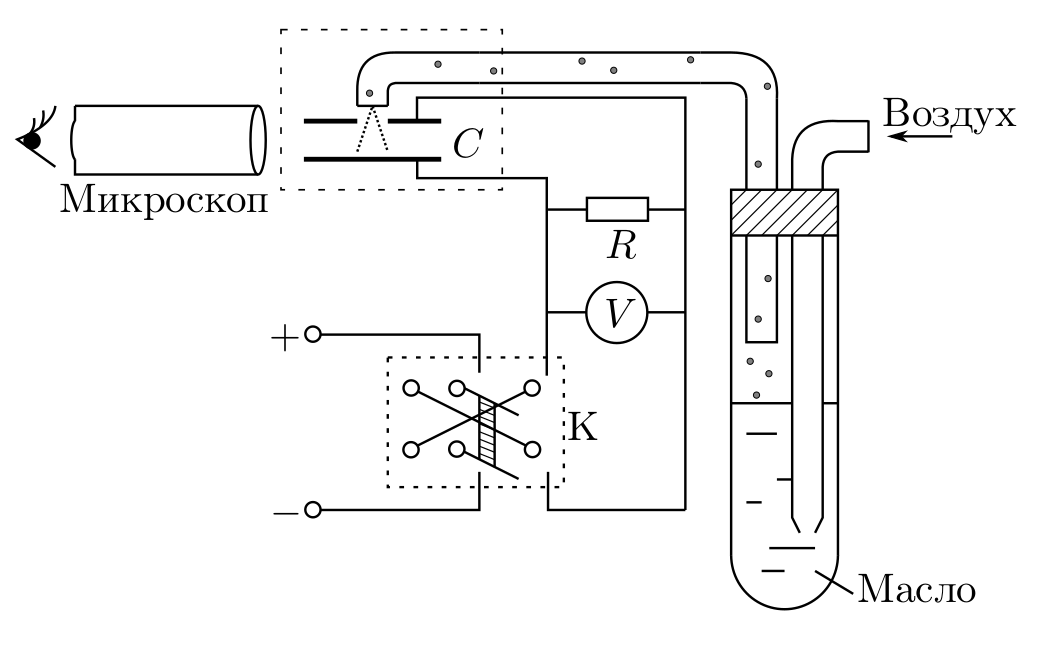
\includegraphics[width = 0.6\textwidth]{images/picture_1.png}
        \end{center}
    \caption{Схема экспериментальной установки}
    \end{figure}

    Схема установки представлена на рисунке 1. Масло разбрызгивается пульверизатором. Капли масла попадают
    в конденсатор $C$ через небольшое отверстие в верхней пластине. При этом часть из них вследствие
    трения об воздух приобретает случайный по величине и знаку электрический заряд.
    
    Напряжение на пластины подаётся от регулируемого выпрямителя и измеряется вольтметром $V$. Ключ
    $K$ позволяет менять направление поля в конденсаторе, чтобы можно было работать как с положительно,
    так и с отрицательно заряженными каплями. При размыкании ключа $K$ конденсатор разряжается через
    дополнительное сопротивление $R \approx 10$ МОм.

    Поскольку исследуемые капли малы, наблюдать из возможно только через микроскоп. В фокальной плоскости
    измерительного микроскопа виден ряд горизонтальных линий, расстояние между которыми постоянно и
    равно $\Delta h = 0.25$ мм. Микроскоп снабжён камерой с выводом изображения на монитор ПК.

\section{Измерения и обработка их результатов}

    \subsection{Постоянные величины}

        \begin{center}
            \captionof{table}{Постоянные величины}
            \begin{tabular}{|c|c|c|c|c|}
                \hline
                l, см & h, мм & U, В & $\eta$, $Па \cdot c$ & $\rho$, кг/$м^3$ \\ \hline
                0.725 &  0.75 &  500 & $1.85 \cdot 10^{-5}$ &              898 \\ \hline
            \end{tabular}
        \end{center}

        \subsection{Измерение заряда капель}

        Считаем, что в формуле \eqref{charge} погрешностями всех величин можно пренебречь по отношению
        к погрешностям $t^{\downarrow}$ и $t^{\uparrow}$, которые равны между собой и равны $\sigma_t = 0.2$ c -
        среднее время реакции человека. Тогда формула \eqref{charge} приобретает вид:
        \begin{equation*}
            q = K\frac{t^{\uparrow} + t^{\downarrow}}{t^{\uparrow} \cdot (t^{\downarrow})^{\frac{3}{2}}},
        \end{equation*}
        где все величины без погрешностей собраны в константе $K$. Таким образом, абсолютная погрешность
        $\sigma_q$ заряда капли определяется по формуле:
        \begin{equation*}
            \sigma_q = \sigma_t \cdot \sqrt{\left(\frac{\partial q}{\partial t^{\uparrow}}\right)^2 + \left(\frac{\partial q}{\partial t^{\downarrow}}\right)^2}
        \end{equation*}
        и равна:
        \begin{equation*}
            \sigma_q = K\sigma_t \cdot \sqrt{\frac{1}{4}\frac{(3t^{\uparrow} + t^{\downarrow})^2}{(t^{\uparrow})^2 \cdot (t^{\downarrow})^5} + \frac{1}{(t^{\uparrow})^4 \cdot t^{\downarrow}}} =
            q \frac{\sigma_t}{t^{\uparrow} + t^{\downarrow}} \sqrt{\left(\frac{1}{2} + \frac{3t^{\uparrow}}{2t^{\downarrow}}\right)^2 + \left(\frac{t^{\downarrow}}{t^{\uparrow}}\right)^2}
        \end{equation*}

        Был измерен заряд 7 капель, для каждой из которых проводилось по 6 серий измерений времени
        движения вверх и вниз. Результаты измерений вместе с расчитанными значениями зарядов и их
        погрешностей приведены в таблице 1.

        Как видно из таблицы, полученные значения заряда лежат в дапазоне $(1.14; 1.35)\cdot 10^{-19}$ Кл.
        Таким образом, величина, которой они кратны - некоторое значение заряда из этого интервала. При этом
        других кратных значений не получено.

    \subsection{Подвешивание капли}

        Пусть в формуле \eqref{charge} $t^{\uparrow} \gg t^{\downarrow}$, тогда выражение для заряда
        принимает вид:
        \begin{equation*}
            q = 9\pi\frac{l}{U}\left(\frac{\eta h}{t^{\downarrow}}\right)^{\frac{3}{2}} \sqrt{\frac{2}{\rho g}}
        \end{equation*}
        Отсюда получаем, что погрешность вычисления по последней формуле равна:
        \begin{equation*}
            \sigma_q = \frac{3}{2}\frac{\sigma_t}{t^{\downarrow}}q
        \end{equation*}
        Было проведено 5 измерений времени падений одной и той же капли при её подвешивании и 
        последующем падении без электрического поля. Результаты измерений вместе с расчитанными 
        значениями заряда и его погрешности приведены в таблице 3.

\section{Вывод}

        Результаты работы таковы, что найденные значения заряда находятся в окрестности некоторой единственной точки.
        Из этого делаем вывод, что заряд всех исследованных масляных капель был пропорционален элементарному с одним и
        тем же коэффициентом. Строго говоря, из этого нельзя делать вывод о величине элементарного заряда, поскольку
        капли могли иметь заряд $ne$, где $n > 1$. Однако, поскольку элементарный заряд всё же известнет, ясно,
        что полученные значения ближе к $e$, чем к кратным ему значениям. Таким образом, величина элементарного
        заряда найдена лишь по порядку, а численный коэффициент порядка единицы не совпадает с ожидаемым даже с учётом
        погрешностей.

\newpage
\section{Приложения}

    \subsection{Таблицы}

    \begin{table}[h]
    \captionof{table}{Измерение заряда капель}
    \begin{tabular}{|c|c|c|c|c|c|c|c|c|c|c|c|}
        \hline
        $t^{\uparrow}$, с & $t^{\downarrow}$, с & \shortstack{q, \\ $10^{-19}$ Кл} & \shortstack{$\sigma_q$, \\ $10^{-19}$ Кл} & \shortstack{q, $10^{-10}$ \\ ед. СГС} & \shortstack{$\sigma_q$, $10^{-10}$ \\ ед. СГС} &
        $t^{\uparrow}$, с & $t^{\downarrow}$, с & \shortstack{q, \\ $10^{-19}$ Кл} & \shortstack{$\sigma_q$, \\ $10^{-19}$ Кл} & \shortstack{q, $10^{-10}$ \\ ед. СГС} & \shortstack{$\sigma_q$, $10^{-10}$ \\ ед. СГС} \\ \hline\hline
        \multicolumn{6}{|c|}{Капля 1}                                                      &         &         &         &                       &       &                      \\ \hline
        34.41   & 24.81   & 1.19    & \multirow{7}{*}{0.01} & 3.58 & \multirow{7}{*}{0.03} &         &         &         &                       &       &                      \\ \hhline{---~-~------}
        34.09   & 24.15   & 1.22    &                       & 3.67 &                       &         &         &         &                       &       &                      \\ \hhline{---~-~------}
        32.56   & 23.88   & 1.28    &                       & 3.85 &                       &         &         &         &                       &       &                      \\ \hhline{---~-~------}
        32.00   & 24.06   & 1.30    &                       & 3.90 &                       &         &         &         &                       &       &                      \\ \hhline{---~-~------}
        32.63   & 23.00   & 1.31    &                       & 3.93 &                       &         &         &         &                       &       &                      \\ \hhline{---~-~------}
        32.33   & 23.85   & 1.29    &                       & 3.88 &                       &         &         &         &                       &       &                      \\ \hhline{---~-~------}
        33.94   & 24.28   & 1.22    &                       & 3.67 &                       &         &         &         &                       &       &                      \\ \hline
        \multicolumn{6}{|c|}{Капля 2}                                                      & \multicolumn{6}{|c|}{Капля 5}                                                      \\ \hline       
        36.42   & 19.50   & 1.32    & \multirow{6}{*}{0.01} & 3.95 & \multirow{6}{*}{0.03} & 42.52   & 17.96   & 1.23    & \multirow{6}{*}{0.01} & 3.68 & \multirow{6}{*}{0.03} \\ \hhline{---~-~---~-~}
        38.64   & 20.18   & 1.23    &                       & 3.68 &                       & 41.21   & 18.30   & 1.24    &                       & 3.72 &                       \\ \hhline{---~-~---~-~}
        40.65   & 20.17   & 1.17    &                       & 3.52 &                       & 39.50   & 18.03   & 1.30    &                       & 3.89 &                       \\ \hhline{---~-~---~-~}
        39.99   & 19.21   & 1.23    &                       & 3.69 &                       & 41.57   & 17.76   & 1.26    &                       & 3.78 &                       \\ \hhline{---~-~---~-~}
        37.50   & 19.75   & 1.27    &                       & 3.82 &                       & 39.71   & 19.58   & 1.22    &                       & 3.67 &                       \\ \hhline{---~-~---~-~}
        41.42   & 19.39   & 1.19    &                       & 3.56 &                       & 38.57   & 19.65   & 1.25    &                       & 3.75 &                       \\ \hline       
        \multicolumn{6}{|c|}{Капля 3}                                                      & \multicolumn{6}{|c|}{Капля 6}                                                      \\ \hline       
        35.58   & 19.83   & 1.33    & \multirow{6}{*}{0.01} & 3.99 & \multirow{6}{*}{0.03} & 36.93   & 20.61   & 1.26    & \multirow{6}{*}{0.01} & 3.77 & \multirow{6}{*}{0.03} \\ \hhline{---~-~---~-~}
        37.72   & 20.06   & 1.26    &                       & 3.77 &                       & 35.08   & 22.41   & 1.25    &                       & 3.74 &                       \\ \hhline{---~-~---~-~}
        38.24   & 21.27   & 1.20    &                       & 3.58 &                       & 37.24   & 23.46   & 1.15    &                       & 3.45 &                       \\ \hhline{---~-~---~-~}
        34.46   & 20.42   & 1.34    &                       & 4.02 &                       & 36.04   & 22.03   & 1.23    &                       & 3.69 &                       \\ \hhline{---~-~---~-~}
        38.15   & 19.79   & 1.25    &                       & 3.76 &                       & 36.17   & 21.59   & 1.24    &                       & 3.72 &                       \\ \hhline{---~-~---~-~}
        38.16   & 21.43   & 1.19    &                       & 3.57 &                       & 36.30   & 22.14   & 1.22    &                       & 3.66 &                       \\ \hline       
        \multicolumn{6}{|c|}{Капля 4}                                                       & \multicolumn{6}{|c|}{Капля 7}                                                      \\ \hline       
        39.16   & 19.49   & 1.24    &    & 3.72 & \multirow{6}{*}{0.03} & 33.41   & 25.07   & 1.22    & \multirow{6}{*}{0.01} & 3.66 & \multirow{6}{*}{0.03} \\ \hhline{---~-~---~-~}
        37.62   & 19.02   & 1.30    &                       & 3.91 &                       & 33.10   & 24.04   & 1.26    &                       & 3.78 &                       \\ \hhline{---~-~---~-~}
        42.78   & 18.92   & 1.18    &                       & 3.53 &                       & 34.05   & 25.95   & 1.17    &                       & 3.52 &                       \\ \hhline{---~-~---~-~}
        37.34   & 19.65   & 1.28    &                       & 3.85 &                       & 35.34   & 24.69   & 1.17    &                       & 3.51 &                       \\ \hhline{---~-~---~-~}
        41.35   & 19.50   & 1.18    &                       & 3.55 &                       & 33.44   & 24.92   & 1.22    &                       & 3.67 &                       \\ \hhline{---~-~---~-~}
        37.93   & 19.80   & 1.26    &                       & 3.78 &                       & 33.03   & 25.97   & 1.21    &                       & 3.62 &                       \\ \hline       
        
        \end{tabular}
    \end{table}

    \begin{center}
    \captionof{table}{Подвешивание капли}
    \begin{tabular}{|c|c|c|c|c|c|}
        \hline
        U, В & $t^{\downarrow}$, с & q, $10^{-19}$ Кл & $\sigma_q$, $10^{-19}$ Кл & q, $10^{-10}$ ед. СГС & $\sigma_q$, $10^{-10}$ ед. СГС \\ \hline\hline
        \multirow{5}{*}{200} & 24.99  &  2.02  &  0.02  & 6.06  & 0.07 \\ \hhline{~-----} 
                             & 26.21  &  1.88  &  0.02  & 5.64  & 0.06 \\ \hhline{~-----}
                             & 26.48  &  1.85  &  0.02  & 5.56  & 0.06 \\ \hhline{~-----}
                             & 25.27  &  1.99  &  0.02  & 5.96  & 0.07 \\ \hhline{~-----}
                             & 24.22  &  2.12  &  0.03  & 6.35  & 0.08 \\ \hline

    \end{tabular}
    \end{center}

\end{document}
